\documentclass[12pt,a4paper]{article}

\usepackage[utf8]{inputenc}
\usepackage[T1]{fontenc}
\usepackage[spanish]{babel}
\usepackage{graphicx}
\usepackage{geometry}
\usepackage{array}
\usepackage{tabularx}
\usepackage{longtable}
\usepackage{float}
\usepackage{hyperref}

\geometry{
    top=2cm,
    bottom=2cm,
    left=2cm,
    right=2cm
}

\graphicspath{{figuras/}{evidencias/}}

\hypersetup{
    colorlinks=true,
    urlcolor=blue,
    linkcolor=black
}

\setlength{\parindent}{0pt}
\setlength{\parskip}{5pt}
\renewcommand{\arraystretch}{1.35}

\begin{document}

% ==================================================
% CARÁTULA
% ==================================================

\begin{titlepage}
\centering

{\Large\textbf{UNIVERSIDAD TÉCNICA ESTATAL DE QUEVEDO}}\\[0.35cm]

{\large Facultad de Ciencias de la Computación y Diseño Digital}\\[0.15cm]

{\large Carrera de Ingeniería de Software}\\[1.2cm]

{\LARGE\textbf{EVALUACIÓN SUMATIVA UNIDAD IV}}\\[0.35cm]

{\large\textbf{Ingeniería de Requisitos}}\\[1.1cm]

\begin{flushleft}

\textbf{Asignatura:} Ingeniería de Requisitos\\[0.35cm]

\textbf{Estudiante:} Díaz Pontón Steven Santiago\\[0.35cm]

\textbf{Nivel:} 4to Nivel\\[0.35cm]

\textbf{Paralelo:} A\\[0.35cm]

\textbf{Fecha:} 11 de agosto de 2026

\end{flushleft}

\vspace{0.8cm}

\textbf{Repositorio de la evaluación}\\[0.3cm]

\href{https://github.com/sdiazp3/EVALUCION_UNIDAD_IV_DIAZ.git}
{\small\texttt{https://github.com/sdiazp3/EVALUCION\_UNIDAD\_IV\_DIAZ.git}}

\vfill

{\large Quevedo -- Ecuador}\\
{\large 2026}

\end{titlepage}

% ==================================================
% EVIDENCIAS DEL CUESTIONARIO DEL SGA
% ==================================================

\section*{Evidencia 1: Resumen del cuestionario}

La siguiente captura corresponde al resumen del cuestionario realizado
en el Sistema de Gestión Académica (SGA).

\vspace{0.5cm}

\begin{center}
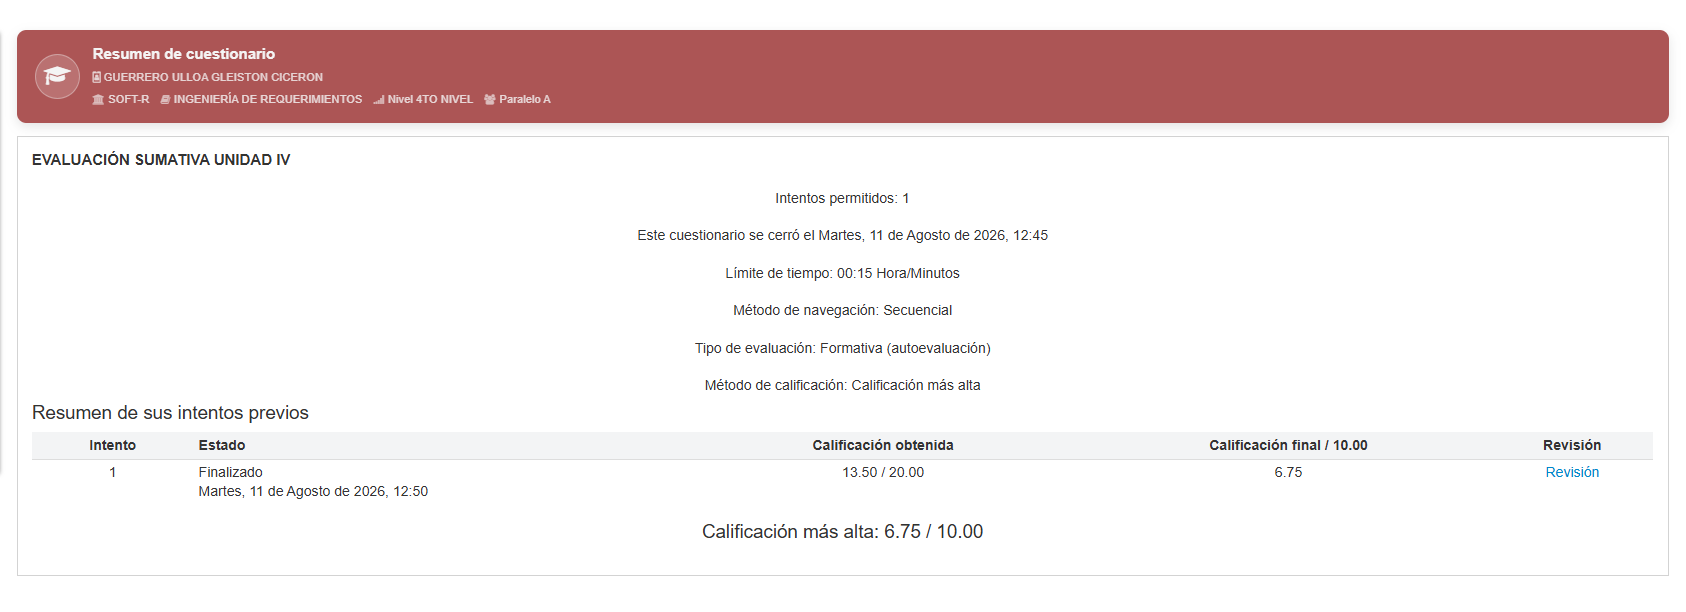
\includegraphics[
    width=\textwidth,
    height=0.72\textheight,
    keepaspectratio
]{resumen_sga.png}
\end{center}

\newpage

\section*{Evidencia 2: Revisión del intento}

La siguiente captura corresponde a la revisión del intento realizado
en el Sistema de Gestión Académica (SGA).

\vspace{0.5cm}

\begin{center}
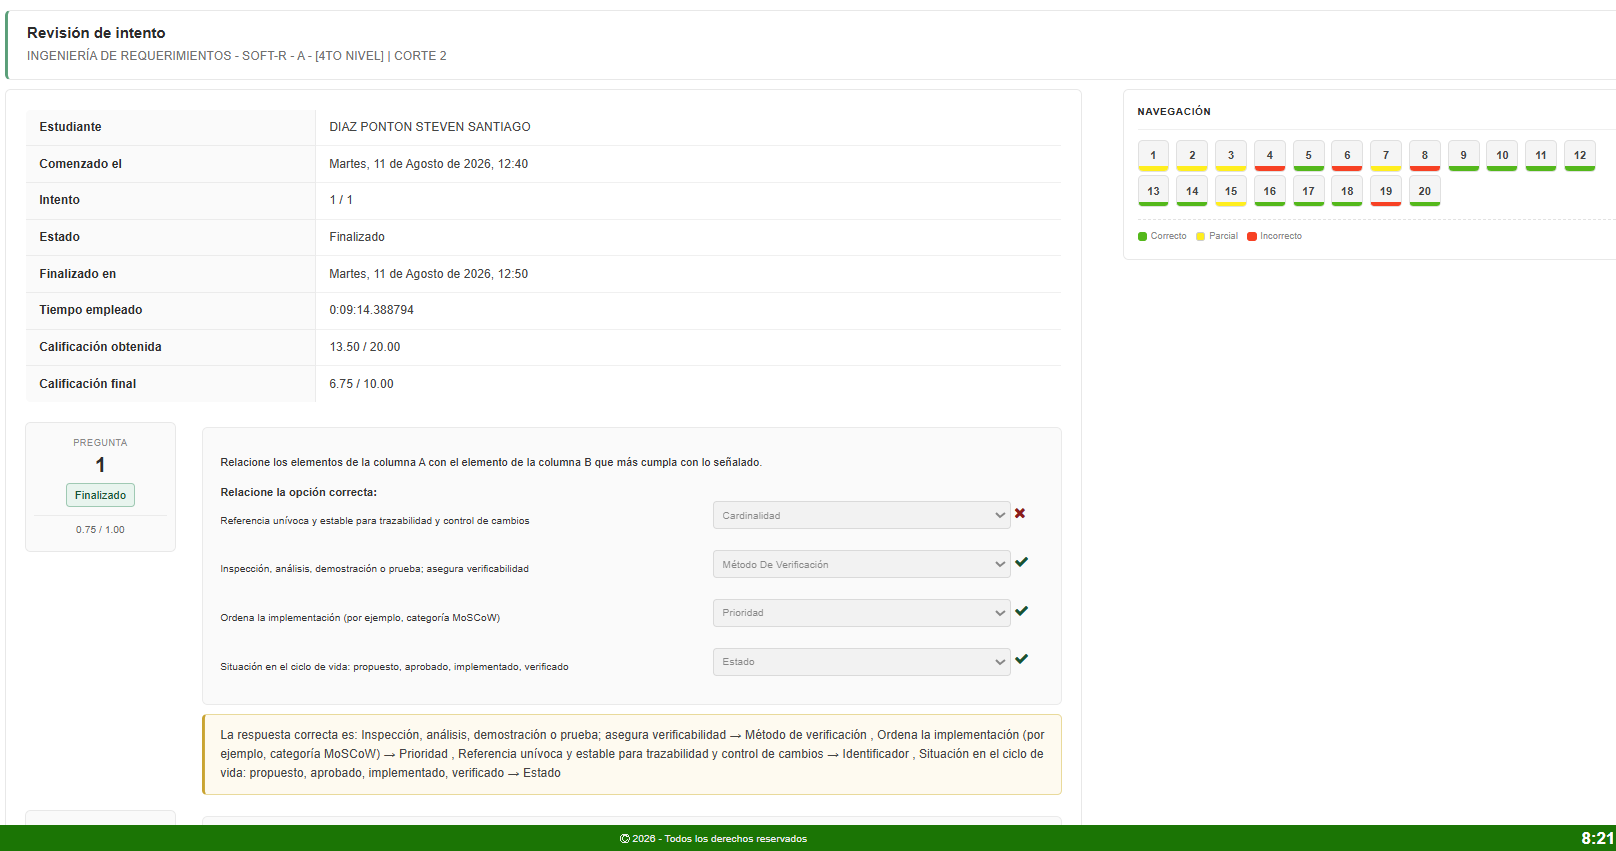
\includegraphics[
    width=\textwidth,
    height=0.72\textheight,
    keepaspectratio
]{revision_intento_sga.png}
\end{center}

\newpage

% ==================================================
% P1
% ==================================================

\section*{P1. Modelo de datos -- Diagrama de clases UML}

\begin{center}
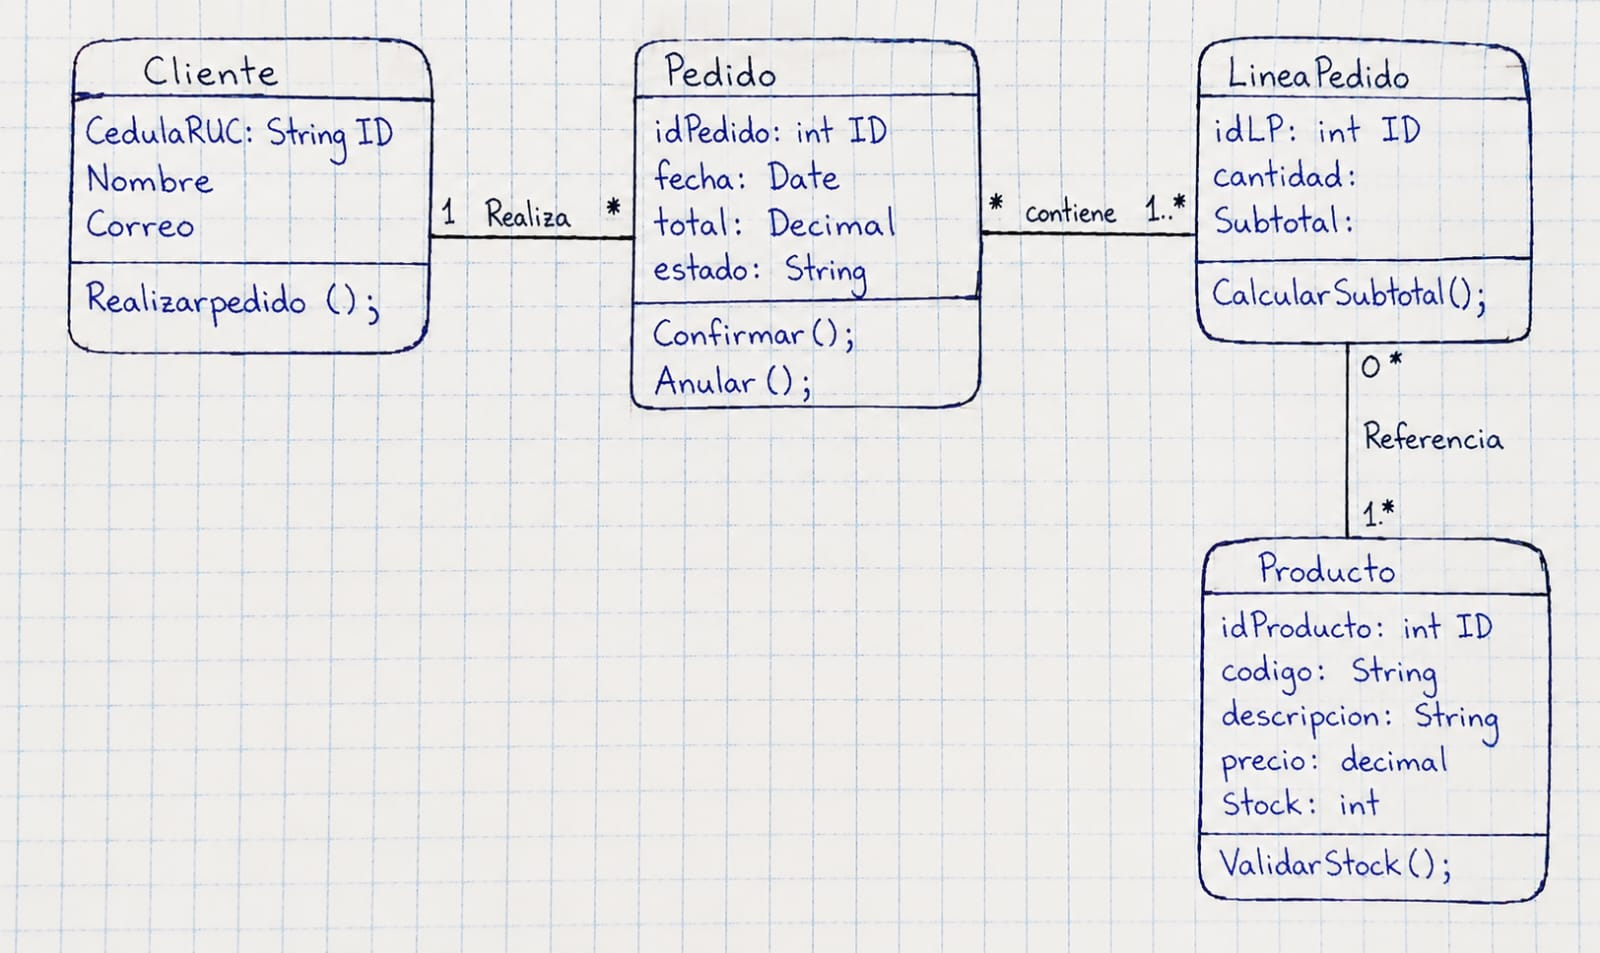
\includegraphics[
    width=\textwidth,
    height=0.75\textheight,
    keepaspectratio
]{P1_diagrama_clases}
\end{center}

\newpage

% ==================================================
% P2
% ==================================================

\section*{P2. Modelo funcional -- Diagrama de actividades}

\begin{center}
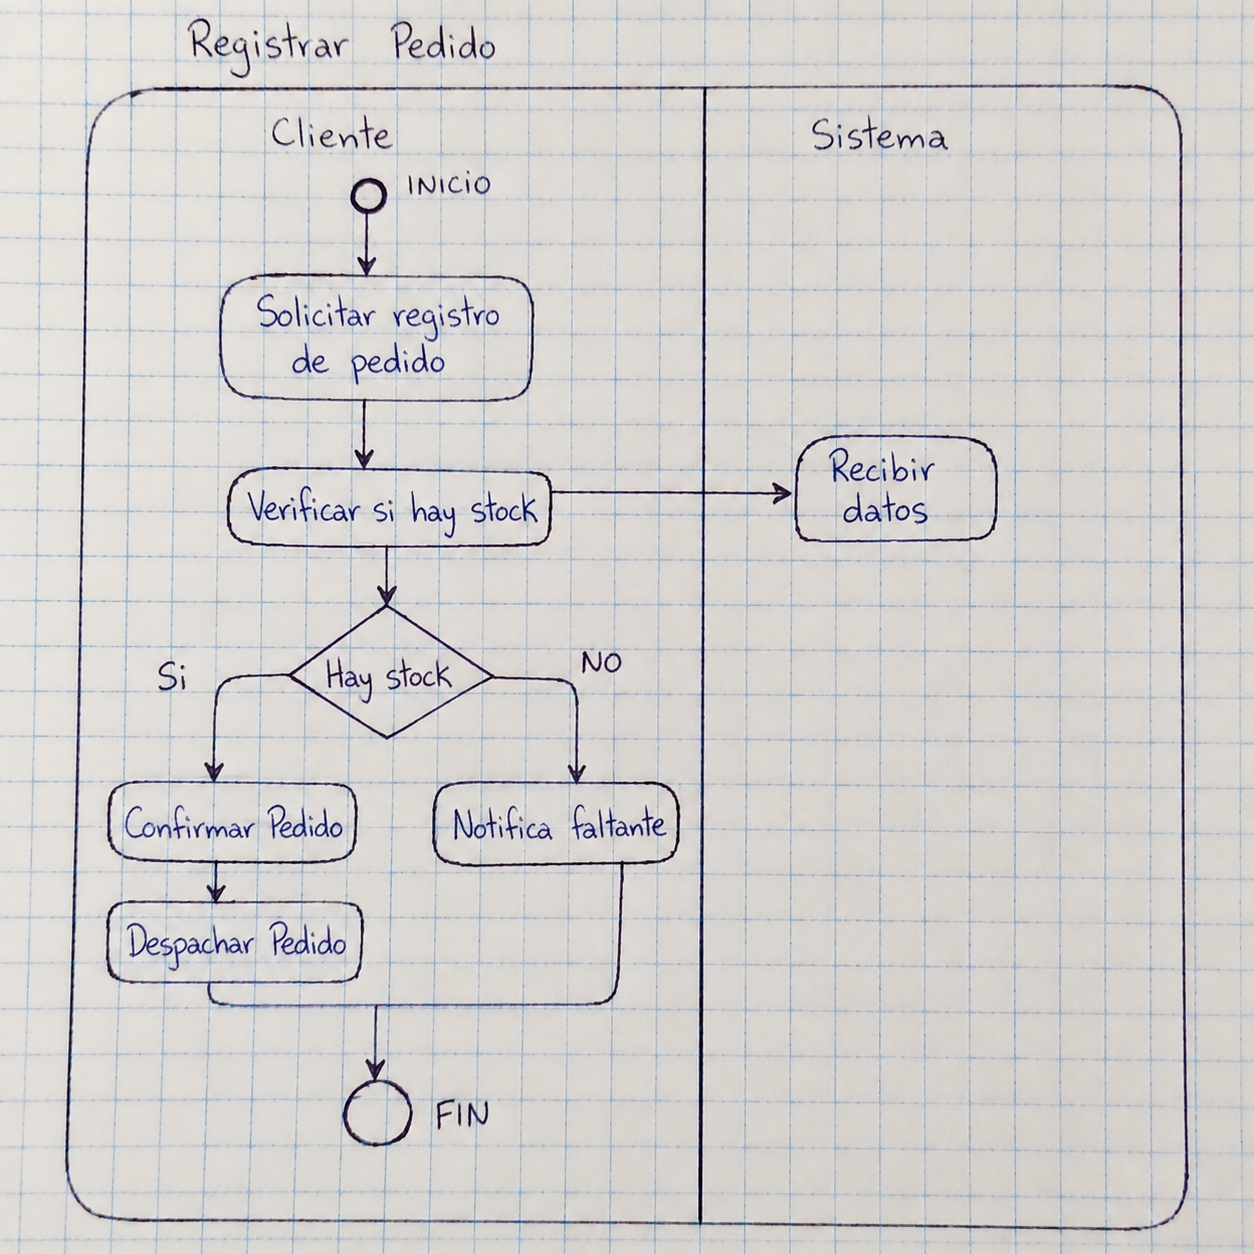
\includegraphics[
    width=\textwidth,
    height=0.75\textheight,
    keepaspectratio
]{P2_diagrama_actividades}
\end{center}

\newpage

% ==================================================
% P3
% ==================================================

\section*{P3. Modelo de comportamiento -- Máquina de estados UML}

\begin{center}
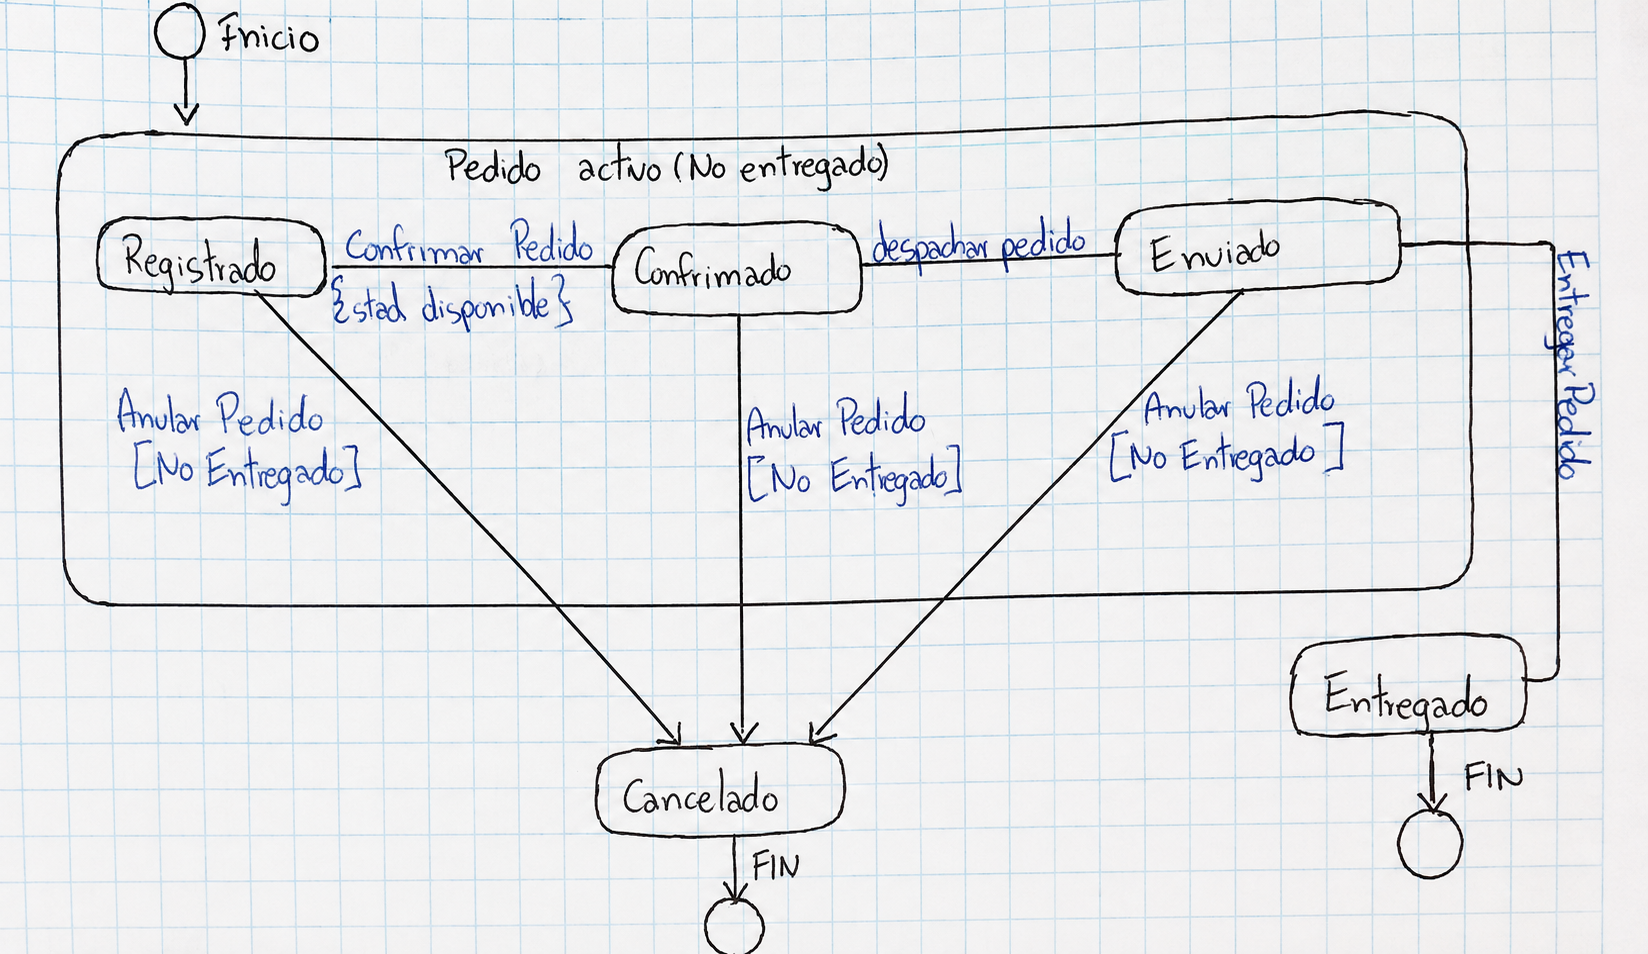
\includegraphics[
    width=\textwidth,
    height=0.75\textheight,
    keepaspectratio
]{P3_maquina_estados}
\end{center}

\newpage

% ==================================================
% P4
% ==================================================

\section*{P4. Consistencia entre las perspectivas}

\begin{table}[H]
\centering
\small

\begin{tabularx}{\textwidth}{
|>{\raggedright\arraybackslash}p{3cm}
|>{\raggedright\arraybackslash}p{4.2cm}
|>{\raggedright\arraybackslash}X|
}
\hline

\textbf{Evento de P3} &
\textbf{Acción correspondiente en P2} &
\textbf{Elemento del P1 afectado} \\
\hline

registrarPedido &
Registrar pedido &
Pedido: idPedido, fecha, total, estado \\
\hline

confirmarPedido &
Confirmar Pedido &
Pedido: estado \\
\hline

despacharPedido &
No aparece en P2 &
Pedido: estado \\
\hline

entregarPedido &
No aparece en P2 &
Pedido: estado \\
\hline

\end{tabularx}
\end{table}

Se documentó un error ya que despachar Pedido no se encuentra en el
diagrama de actividades, para su corrección agregaré despachar Pedido
bajo la consigna de confirmar Pedido, ya actualmente aquel error fue
corregido en el diagrama de actividades que se encuentra en P2.

% ==================================================
% P5
% ==================================================

\section*{P5. Especificación de requisitos con esquema de atributos}

\begin{table}[H]
\centering
\small

\begin{tabularx}{\textwidth}{
|>{\raggedright\arraybackslash}p{1.5cm}
|>{\raggedright\arraybackslash}X
|>{\raggedright\arraybackslash}p{4cm}|
}
\hline

\textbf{ID} &
\textbf{Requisito Descripción} &
\textbf{Característica normas ISO} \\
\hline

RF-01 &
El sistema deberá permitir registrar un pedido asociado a un cliente
con una o más líneas de pedido. &
Registrar Pedido \\
\hline

RF-02 &
El sistema deberá verificar la disponibilidad del stock antes de
confirmar un producto. &
Verificar Stock \\
\hline

RNF-01 &
El sistema deberá registrar un pedido en un tiempo menor a 3 segundos. &
Eficiencia de desempeño $<3s$ \\
\hline

RNF-02 &
El sistema deberá proteger los datos personales del cliente mediante
cifrado durante su transmisión. &
Seguridad; 99\% \\
\hline

\end{tabularx}
\end{table}

En cuanto a la métrica de seguridad se le asigna un valor de al menos
99\% ya que nada es completamente seguro en esta vida y puede llegar
a ocurrir un error en la transmisión.

% ==================================================
% ESQUEMA DE ATRIBUTOS
% ==================================================

\subsection*{Esquema de Atributos}

\begin{table}[H]
\centering
\small

\begin{tabularx}{\textwidth}{
|>{\raggedright\arraybackslash}p{2.7cm}
|>{\centering\arraybackslash}X
|>{\centering\arraybackslash}X
|>{\centering\arraybackslash}X
|>{\centering\arraybackslash}X|
}
\hline

\textbf{Identificador} &
\textbf{RF-01} &
\textbf{RF-02} &
\textbf{RNF-01} &
\textbf{RNF-02} \\
\hline

Prioridad &
Alta &
Alta &
Media &
Alta \\
\hline

Estado &
Propuesto &
Propuesto &
Propuesto &
Propuesto \\
\hline

Fuente &
Caso Práctico &
Caso Práctico &
Caso Práctico &
Caso Práctico \\
\hline

Estabilidad &
Alta &
Alta &
Alta &
Alta \\
\hline

Versión &
1.0 &
1.0 &
1.0 &
1.0 \\
\hline

Verificación &
Prueba Funcional &
Prueba Funcional &
Prueba Funcional &
Prueba Funcional \\
\hline

\end{tabularx}
\end{table}

% ==================================================
% P6
% ==================================================

\section*{P6. Priorización MoSCoW}

\begin{table}[H]
\centering
\small

\begin{tabularx}{\textwidth}{
|>{\raggedright\arraybackslash}p{3.4cm}
|>{\centering\arraybackslash}p{2.2cm}
|>{\raggedright\arraybackslash}X|
}
\hline

\textbf{Requisito} &
\textbf{MoSCoW} &
\textbf{Justificación} \\
\hline

RF-01 Registrar Pedido &
Must Have &
Es la función principal del sistema, sin él no se pueden gestionar pedidos. \\
\hline

RF-02 Verificar Stock &
Must Have &
Es necesario para evitar la confirmación de pedidos cuando no hay
stock del producto. \\
\hline

RNF-01 Tiempo de Respuesta &
Should Have &
Es importante que el registro sea rápido pero el sistema puede
funcionar aunque no alcance ese tiempo. \\
\hline

RNF-02 Seguridad &
Must Have &
Es importante mantener la seguridad del cliente. \\
\hline

\end{tabularx}
\end{table}

% ==================================================
% P7
% ==================================================

\section*{P7. Validación por inspección (lista de comprobación 29148)}

\begin{table}[H]
\centering
\footnotesize

\begin{tabularx}{\textwidth}{
|c|c|c|c|c|c|>{\raggedright\arraybackslash}X|
}
\hline

\textbf{Req.} &
\textbf{No ambiguo} &
\textbf{Completo} &
\textbf{Singular} &
\textbf{Verificable} &
\textbf{Factible} &
\textbf{Defecto} \\
\hline

RF-01 &
Sí &
Sí &
Sí &
Sí &
Sí &
Ninguno \\
\hline

RF-02 &
Sí &
Sí &
Sí &
Sí &
Sí &
Ninguno \\
\hline

RNF-01 &
No &
No &
Sí &
Sí &
Sí &
No especifica bajo qué condiciones se medirán los 3s \\
\hline

RNF-02 &
No &
No &
Sí &
No &
Sí &
No especifica qué cifrado o mecanismo comprueba la protección \\
\hline

\end{tabularx}
\end{table}

\subsection*{RNF-01 Corregido -- V1.1}

El sistema deberá registrar un pedido en un tiempo menor a 3 segundos,
bajo una carga de hasta 50 usuarios concurrentes.

\subsection*{RNF-02 Corregido -- V1.1}

El sistema deberá transmitir el 99\% de los datos personales del cliente
mediante una conexión cifrada HTTPS/TLS.

% ==================================================
% P8
% ==================================================

\section*{P8. Pruebas de aceptación trazadas}

\begin{table}[H]
\centering
\small

\begin{tabularx}{\textwidth}{
|>{\centering\arraybackslash}p{1.3cm}
|>{\centering\arraybackslash}p{1.5cm}
|>{\centering\arraybackslash}p{2.1cm}
|>{\raggedright\arraybackslash}p{3.6cm}
|>{\raggedright\arraybackslash}X|
}
\hline

\textbf{Prueba} &
\textbf{Requisito} &
\textbf{Tipo} &
\textbf{Entradas} &
\textbf{Criterio de éxito} \\
\hline

PA-01 &
RF-01 &
Funcional &
Cliente válido, 2 productos y cantidades &
El pedido se registra correctamente con una o más líneas de pedido \\
\hline

PA-02 &
RF-02 &
Funcional &
Producto solicitado: 10 unidades; stock 5 &
El sistema detecta que no existe stock suficiente y no confirma el pedido \\
\hline

PA-03 &
RNF-01 &
No Funcional &
Registro de pedidos con hasta 50 usuarios &
El pedido se registra en menos de 3 segundos \\
\hline

PA-04 &
RNF-02 &
No Funcional &
Transmisión de datos personales de un cliente &
El 99\% de los datos personales se transmiten mediante HTTPS/TLS \\
\hline

\end{tabularx}
\end{table}

% ==================================================
% P9
% ==================================================

\section*{P9. Matriz de trazabilidad}

\begin{table}[H]
\centering
\footnotesize

\begin{tabularx}{\textwidth}{
|>{\raggedright\arraybackslash}p{2.7cm}
|>{\raggedright\arraybackslash}p{1.8cm}
|>{\raggedright\arraybackslash}X
|>{\centering\arraybackslash}p{1.8cm}
|>{\centering\arraybackslash}p{2.1cm}
|>{\centering\arraybackslash}p{1.3cm}|
}
\hline

\textbf{Requisito} &
\textbf{Fuente} &
\textbf{Modelo relacionado} &
\textbf{Prueba aceptación} &
\textbf{Dependencia Horizontal} &
\textbf{¿Huérfano?} \\
\hline

RF-01 Registrar pedido &
Caso Práctico &
P1 clases, P2 Actividades &
PA-01 &
-- &
No \\
\hline

RF-02 Verificar stock &
Caso Práctico &
P1 clases, P2 Actividades, P3 estados &
PA-02 &
RF-01 &
No \\
\hline

RNF-01 Rendimiento $<3s$ &
Caso Práctico &
P2 Actividades &
PA-03 &
RF-01 &
No \\
\hline

RNF-02 Seguridad datos &
Caso Práctico &
P1 Clases &
PA-04 &
RF-01 &
No \\
\hline

\end{tabularx}
\end{table}

% ==================================================
% P10
% ==================================================

\section*{P10. Gestión de cambio y línea base}

\subsection*{1. Solicitud de cambio -- RFC-01}

\begin{table}[H]
\centering
\small

\begin{tabularx}{0.92\textwidth}{
|>{\raggedright\arraybackslash}p{4cm}
|>{\raggedright\arraybackslash}X|
}
\hline

\textbf{Campo} &
\textbf{Información} \\
\hline

ID &
RFC-01 \\
\hline

Requisito afectado &
RNF-01 \\
\hline

Versión actual &
1.0 \\
\hline

Cambio solicitado &
Reducir el tiempo máximo de registro de 3 a 2s \\
\hline

Motivo &
Mejorar la rapidez del registro de pedidos \\
\hline

Estado &
En evaluación \\
\hline

\end{tabularx}
\end{table}

\subsection*{2. Análisis de Impacto}

\begin{table}[H]
\centering
\small

\begin{tabularx}{0.92\textwidth}{
|>{\raggedright\arraybackslash}p{4cm}
|>{\raggedright\arraybackslash}X|
}
\hline

\textbf{Elemento} &
\textbf{Impacto} \\
\hline

RNF-01 &
Cambiar umbral de 3s a 2s \\
\hline

PA-03 &
Cambiar criterio de éxito a menos de 2s \\
\hline

P2-Actividades &
Se mantiene relacionado con RNF-01 \\
\hline

Matriz P9 &
Actualizar versión de RNF-01 \\
\hline

ERS &
Actualizar requisito \\
\hline

\end{tabularx}
\end{table}

\subsection*{3. Decisión del CCB}

\textbf{Decisión: APROBADA.}

El CCB aprueba la mejora de cambio para mejorar la eficiencia del Sistema.

\subsection*{4. Actualización de Versión}

RNF-01 v1.0 $\rightarrow <3$ Segundos

\vspace{0.2cm}

RNF-01 v1.1 $\rightarrow <2$ Segundos

\end{document}